\section{Representación gráfica del arreglo}

La arquitectura de este arreglo se explica en las secciones~\ref{sec:diseno-arreglo} y~\ref{sec:archivo-indexado}; 
para evitar redundancia en esta seccion no se explicara la justificacion aun.

\begin{figure}[h]
    \centering
    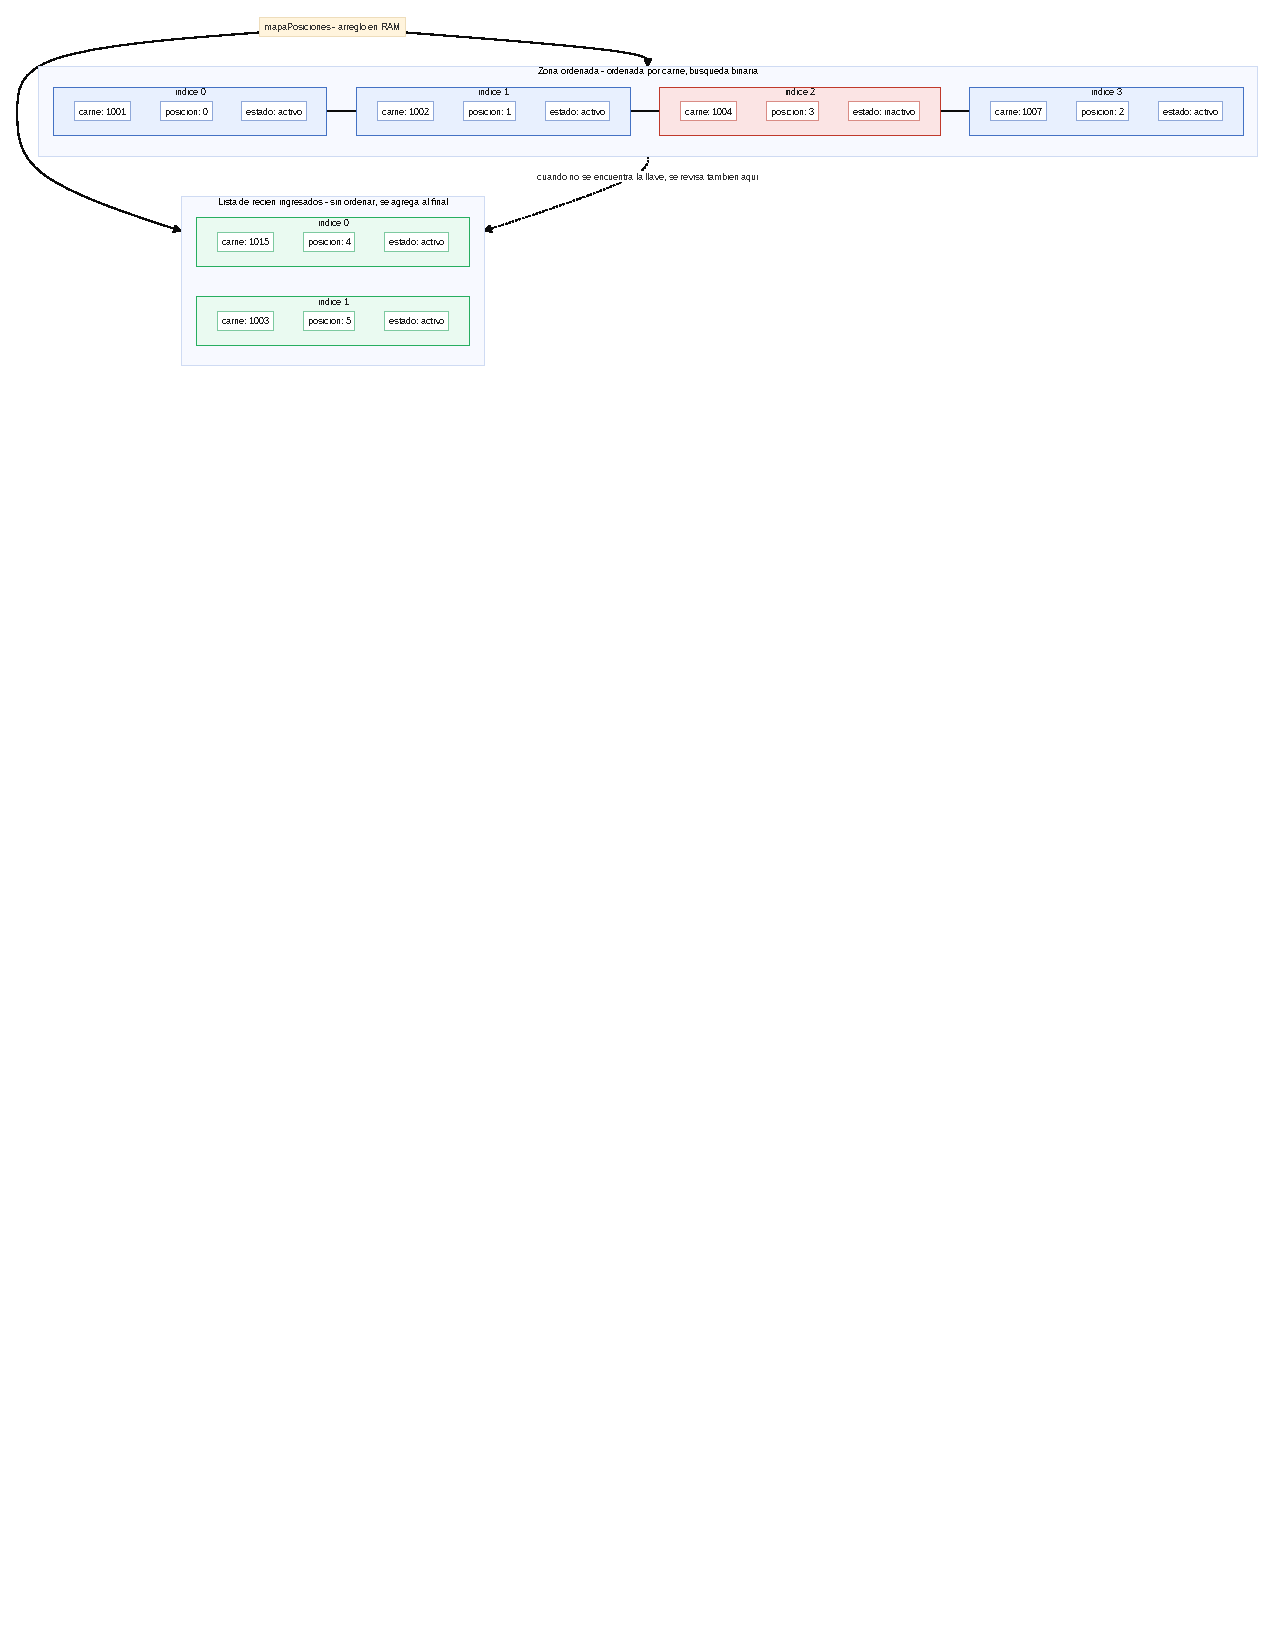
\includegraphics[width=0.85\textwidth]{../diagramas/output/mapa-posiciones-ram.pdf}
    \caption{El mapa de posiciones como arreglo en RAM}
    \label{fig:mapa-posiciones-ram}
\end{figure}

La figura~\ref{fig:mapa-posiciones-ram} muestra las dos zonas del mapa por carné descritas en la subsección~\ref{sec:mapa-por-carne} 
aparecen como dos arreglos separados: 
\begin{enumerate}
    \item La \textbf{zona ordenada} (índices 0 a 3)
    \item La \textbf{lista de recién ingresados} (índice 0, con el carné 1015 que todavía no fue integrado)
\end{enumerate}

Cada celda, en cualquiera de las dos zonas, tiene la misma composición de tres campos justificada en la subsección~\ref{sec:composicion-entrada}. 
La celda en rojo (carné 1004) es el mismo ejemplo de estado inactivo usado en la sección~\ref{sec:archivo-indexado}.

\newpage

\begin{figure}[h]
    \centering
    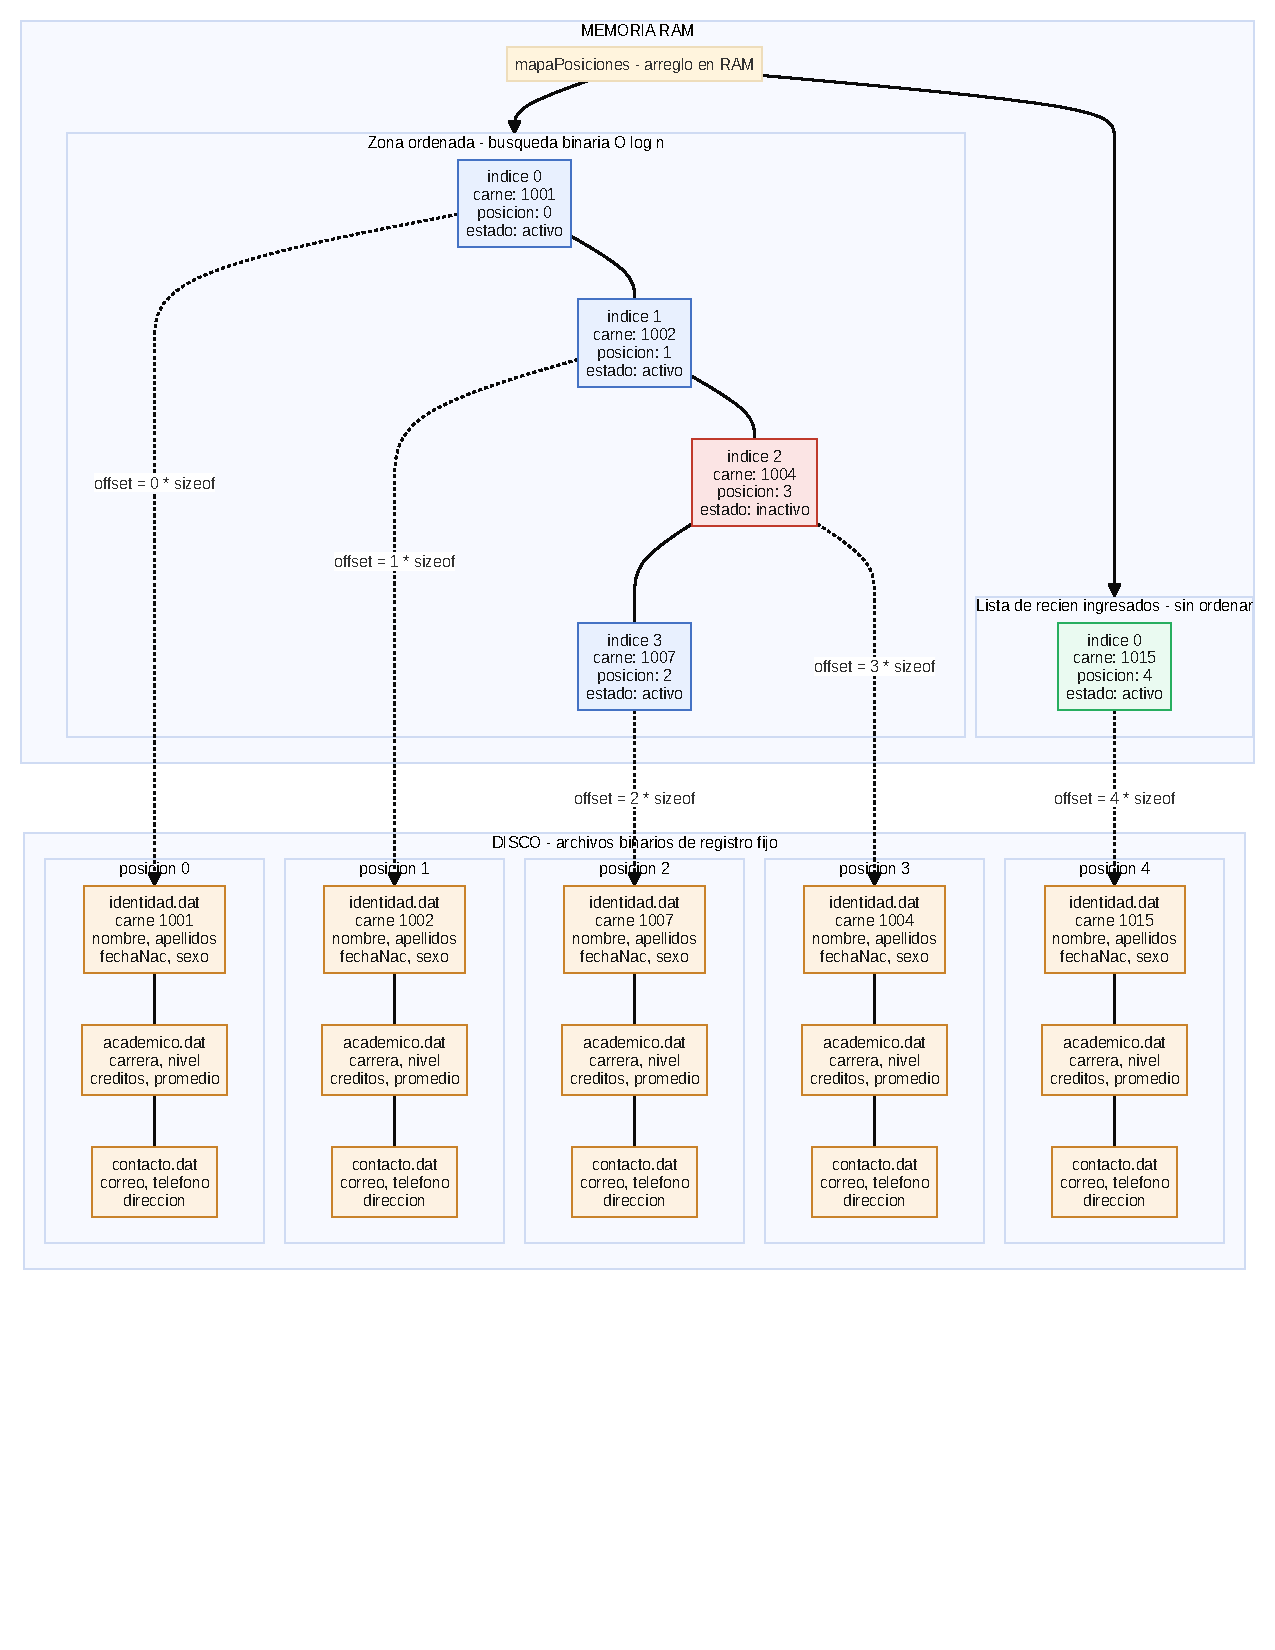
\includegraphics[width=0.95\textwidth]{../diagramas/output/arreglo-estudiantes.pdf}
    \caption{Relación entre el mapa de posiciones en RAM y los archivos en disco}
    \label{fig:arreglo-estudiantes}
\end{figure}

La figura~\ref{fig:arreglo-estudiantes} agrega los tres archivos en disco (sección~\ref{sec:archivo-secuencial}) a la misma estructura de la
figura anterior. Las flechas punteadas son el cálculo de \texttt{offset} de la sección~\ref{sec:archivo-secuencial} aplicado a
cada entrada del mapa: 
\begin{itemize}
    \item El carné 1007 (zona ordenada, índice 3) apunta a la posición 2 en disco
    \item El carné 1004 (inactivo) apunta a la posición 3
    \item El carné 1015 (lista de recién ingresados) apunta a la posición 4, la más reciente
\end{itemize}

Las tres columnas de cada posición (\texttt{identidad.dat}, \texttt{academico.dat}, \texttt{contacto.dat}) ilustran que comparten 
índice sin necesitar una llave adicional entre ellas, también justificado en la sección~\ref{sec:archivo-secuencial}.
